%! Author = bedlamzd
%! Date = 16.02.2021

% Preamble
\documentclass[14pt]{extarticle}

%! Author = bedlamzd
%! Date = 16.02.2021

\usepackage{fontspec}
\usepackage{polyglossia}
\defaultfontfeatures{Ligatures=TeX}
\setdefaultlanguage{russian}
\setotherlanguage{english}
\setmainfont{PT Astra Serif}
\newfontfamily{\latinfont}{PT Astra Serif}
\newfontfamily{\cyrillicfont}{PT Astra Serif}
\newfontfamily{\cyrillicfonttt}{FreeMono}

\usepackage{geometry}

\usepackage{amsmath}
\usepackage{amssymb}
\usepackage{amsfonts}
\usepackage{graphicx}
\usepackage{float}
\usepackage{wrapfig}
\usepackage[caption=false]{subfig}

\geometry{right=20mm}
\geometry{left=20mm}
\geometry{top=20mm}
\geometry{bottom=20mm}

\usepackage{indentfirst}
\usepackage[outputdir=out]{minted}

\renewcommand{\theFancyVerbLine}{\ttfamily{\normalsize\oldstylenums{\arabic{FancyVerbLine}}}}

\newminted{python}{autogobble, linenos, fontsize=\small, xleftmargin=2\parindent}
\newmintinline{python}{fontsize=\small}
\newmintedfile{python}{autogobble, linenos, fontsize=\small, xleftmargin=2\parindent,
breakanywhere, breaklines}

\renewcommand{\thesubsection}{\arabic{subsection}}

\graphicspath{{../img/}}



% Document
\begin{document}
    \begin{center}
        \Large Лабораторная работа 2. Введение в нейронные сети с Python
    \end{center}
    \begin{flushleft}
        \textbf{Имя:} Борисов Максим

        \vspace{1em}
        \textbf{Номер в ИСУ:} 225169

        \vspace{1em}
        \textbf{Группа:} R41341C
    \end{flushleft}

    \section*{Задание}
    Реализовать нейронную сеть, которая способна распознавать рукописные цифры
    на изображении. Использовать датасет MNIST.

    \vspace{1em}
    Необходимо
    \begin{enumerate}
        \item Импортировать библиотеки
        \item Реализовать функцию инициализации параметров сети
        \item Реализовать функцию инициализации весов сети
        \item Реализовать функцию расчёта выходного значения сети
        \item Реализовать функцию обучения нейронной сети
        \item Реализовать функцию валидации нейронной сети
        \item Реализовать функцию вывода изображений из датасета
        \item Обучить сеть и провести валидацию
    \end{enumerate}

    \pagebreak

    \paragraph*{Замечание}
    В работе для удобства нейронная сеть реализована через класс, соответственно представленный код
    по структуре и исполнению отличается от предложенного в материалах для подготовки.

    \subsection{Импортирование библиотек}
    \pythonfile[firstline=1, lastline=6]{../src/main.py}
    Библиотека \pythoninline/typing/ необходима для указания сигнатур функций для удобства работы в IDE.

    Библиотека \pythoninline/csv/ используется для чтения данных из датасета.

    \subsection{Реализация функции инициализации параметров сети}
    Функция для получения параметров сети. Имеет флаг \pythoninline/default/ при котором возвращает
    значения параметров по умолчанию без необходимости вводить их с клавиатуры.
    \pythonfile[firstline=74, lastline=91]{../src/main.py}

    Эти данные передаются в конструктор класса \pythoninline/NetworkMNIST/, который также инициализирует
    веса случайными значениями. Однако ничто не мешает их переопределить.
    \pythonfile[firstline=9, lastline=23]{../src/main.py}

    \subsection{Реализация функции инициализации весов}
    \pythonfile[firstline=25, lastline=27]{../src/main.py}
    Инициализировать веса одинаковыми значениями нет смысла, в таком случае сеть будет плохо обучаться.
    В случае со всеми весами равными 0.5 данная сеть в принципе всегда выдаёт на выходе единицы и не обучается вовсе (веса
    не изменяются).

    Однако если инициализировать веса случайным образом (с зерном 42) и попробовать без обучения предсказать число для
    изображения номер 6 в датасете, то ответ будет 1.

    \subsection{Реализация функции расчёта выходного значения сети}
    \pythonfile[firstline=29, lastline=34]{../src/main.py}

    \subsection{Реализация функции обучения сети}
    \pythonfile[firstline=36, lastline=45]{../src/main.py}

    \subsection{Реализация функции валидации сети}
    \pythonfile[firstline=47, lastline=55]{../src/main.py}

    \subsection{Реализация функции вывода изображений из датасета}
    \pythonfile[firstline=94, lastline=98]{../src/main.py}
    \begin{figure}[H]
        \centering
        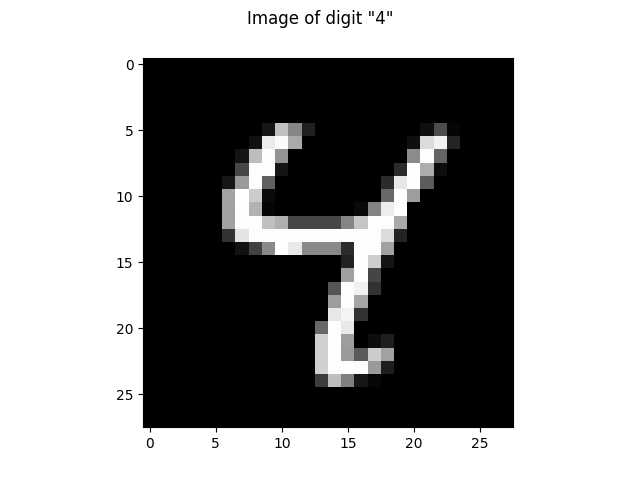
\includegraphics{random_image.png}
        \caption{Изображение из датасета соответствующее варианту}
    \end{figure}

    \subsection{Обучение и валидация сети}
    \pythonfile[firstline=120, lastline=129]{../src/main.py}
    Цифра соответствующая шестому (по номеру варианта), считая от нуля, элементу датасета это 4.

    \pagebreak
    \section*{Полный код}
    \pythonfile{../src/main.py}

\end{document}
